%%%%%%%%%%%%%%%%%%%%%%%%%%%%%%%%%%%%%%%%%%%%%%%%%%%%%%%%%%%%%%%%%%
%%%%%%%% ICML 2014 EXAMPLE LATEX SUBMISSION FILE %%%%%%%%%%%%%%%%%
%%%%%%%%%%%%%%%%%%%%%%%%%%%%%%%%%%%%%%%%%%%%%%%%%%%%%%%%%%%%%%%%%%

% Use the following line _only_ if you're still using LaTeX 2.09.
%\documentstyle[icml2014,epsf,natbib]{article}
% If you rely on Latex2e packages, like most moden people use this:
\documentclass{article}

% use Times
\usepackage{times}
% For figures
\usepackage{graphicx} % more modern
\usepackage{tabulary}
%\usepackage{epsfig} % less modern
\usepackage{subfigure} 

% For citations
\usepackage{natbib}

% For algorithms
\usepackage{algorithm}
\usepackage{algorithmic}

% As of 2011, we use the hyperref package to produce hyperlinks in the
% resulting PDF.  If this breaks your system, please commend out the
% following usepackage line and replace \usepackage{icml2014} with
% \usepackage[nohyperref]{icml2014} above.
\usepackage{hyperref}

% Packages hyperref and algorithmic misbehave sometimes.  We can fix
% this with the following command.
\newcommand{\theHalgorithm}{\arabic{algorithm}}

% Employ the following version of the ``usepackage'' statement for
% submitting the draft version of the paper for review.  This will set
% the note in the first column to ``Under review.  Do not distribute.''
\usepackage[accepted]{icml2014} 


% The \icmltitle you define below is probably too long as a header.
% Therefore, a short form for the running title is supplied here:
\icmltitlerunning{Predicting progression of Alzheimer's Disease}

\begin{document} 

\twocolumn[
\icmltitle{Predicting progression of Alzheimer's Disease with CSF biomarker, genotype, and MRI data}

% It is OKAY to include author information, even for blind
% submissions: the style file will automatically remove it for you
% unless you've provided the [accepted] option to the icml2014
% package.
\icmlauthor{Josh Tycko}{joshtycko@gmail.com}
\icmlauthor{Spencer Penn}{spenn321@gmail.com}
\icmlauthor{Juan Jose Lopez Delgado}{juanlop@seas.upenn.edu}

% You may provide any keywords that you 
% find helpful for describing your paper; these are used to populate 
% the "keywords" metadata in the PDF but will not be shown in the document
\icmlkeywords{Alzheimer's disease, machine learning, ensemble methods, genotype}

\vskip 0.3in
]

\begin{abstract} 
%REWRITE THE ABSTRACT AT THE END!!!!!!
Machine learning algorithms have the potential to predict Alzheimer's disease (AD) progression by analyzing large clinical, genomic, biomarker, and MRI datasets. None of these data types has a standard predictor alone. Using data for 800 patients from the ADNI1 database, we implemented three strategies to generate clinically useful predictions. After attempting two strategies based on the Mini-Mental State Examination measure of cognition, we determined to implement a more clinically relevant strategy, quantifying changes in cognition with the Alzheimer's Disease Assessment Scale Cognitive Subscale (ADAS-cog). A decision tree learner was optimal because it can handle mixed data and missing values, while returning interpretable results that can be relatively transparent in the clinic. We used varying combinations of data types and feature selection methods to gain insight into which features may be most informative for AD physicians to analyze in the future.
%REWRITE THE ABSTRACT AT THE END!!!!!!%REWRITE THE ABSTRACT AT THE END!!!!!!
%REWRITE THE ABSTRACT AT THE END!!!!!!
\end{abstract} 


\section{Introduction}
Alzheimer's disease (AD) is predicted to affect 1 in 85 people globally by 2050, causing dementia and eventual death. Care in the US costs \$100 billion annually, and the available drugs can only help relieve some symptoms \cite{duthey13}.

\subsection{Motivation}
It is currently difficult to predict the progression of AD, and it often progresses undiagnosed for years. Machine learning algorithms have the potential to assist doctors and patients by accurately predicting disease progression based on clinical,  genetic, MRI, and cerebrospinal fluid (CSF) biomarker data, which could enable accurate, early diagnoses. In addition, such an algorithm could potentially accelerate drug development by helping pharmaceutical companies better recruit patients with progressing dementia who stand to benefit from the drugs. Currently, patient recruitment for clinical trials is a major obstacle to drug development, in part because it is difficult for doctors to discern which of their cognitively normal (CN) or mildly cognitively impaired (MCI) patients are likely to develop more significant dementia in the future \cite{watson14}.

\subsection{Related work} Since the causes of AD are currently unknown and there are no laboratory tests that can accurately perform a diagnosis, AD progression is quantified with psychological tests like the mini-mental state examination (MMSE) - a questionnaire used to measure cognitive impairment. This set of 30 questions was developed in 1975 and remains the most widely used test by doctors \cite{carolan07}. The Alzheimer's Disease Assessment Scale Cognitive Subscale (ADAS-cog) is another such test, developed in 1984, and is now the standard assessment used in clinical trials \cite{meade05}.

Machine learning algorithms have been used on ADNI data with varying success to predict the change in MMSE and ADAS-cog \cite{stonnington10}.
Interestingly, in a large study comparing approaches, no single algorithm was superior across all AD datasets, particularly when progression was measured up to varying time points \cite{umer11}


\section{Materials \& Methods}
\subsection{Data} Data used in the preparation of this article were obtained from the Alzheimer's Disease Neuroimaging Initiative (ADNI) database (adni.loni.usc.edu). First, we used data that was collected over 2 years in 767 patients, including mental examinations and genotype in order to predict the progression of AD over time. Progression is quantified by the change in MMSE score over a 24 month period $(\Delta$MMSE$)$.\\

We also enlarged the data set to include the %XXX
patients for whom the ADAS-cog score was measured, and then quantified progressing disease as a change in ADAS greater than 4 points after a time of 6 months or later. For these patients, we additionally considered MRI and CSF biomarker data. The MRI images were analyzed at UCSF with the Free Surfer software package to quantify thickness, volume, and surface area of brain regions. The CSF biomarker analysis was performed at UPenn, and includes key markers associated with AD: amyloid beta, tau, and p-tau 181. 


\subsection{Learning Approach} 

First, we split the data for 767 patients into training and testing sets. As we were interested in creating an algorithm that could predict disease progression quantitatively, we applied a linear regression to predict $(\Delta$MMSE$)$. Since several of our features were categorical data, we used dummy variables to break them into multiple features that could be weighted accordingly in the model.\\

Next, we developed a system to categorize patients by Normal Cognition, Mild Impairment, Moderate Impairment, and Severe Impairment; based on MMSE scores (Table 1). We used these classes to begin applying classification algorithms, including SVM, Decision Tree, and Naive Bayes. 

%Updated
\begin{flushleft}
\begin{table}[h]
\caption{Interpretations of the MMSE Score, ranging from full normal cognition to sever impairment -- which is closely correlated with the presence of dementia. We used this breakdown for classification style ML methods.}
\label{sample-table}
\vskip 0.15in
\begin{center}
\begin{small}
\begin{sc}
\begin{tabular}{lcccr}
\hline
\abovespace
\belowspace
Cognitive States & MMSE Score (out of 30) \\
\hline
\abovespace
\belowspace
Normal Cognition    & $>$ 27 points \\
\belowspace
Mild Impairment & 27 - 23 points  \\
\belowspace
Moderate Impairment    &  23 - 20 points  \\
\belowspace
Severe Impairment     &  $<$ 20 points  \\

\hline
\end{tabular}
\end{sc}
\end{small}
\end{center}
\vskip -0.1in
\end{table}

\end{flushleft}

Then, we presented our results to ADNI scientists at UPenn and gained further insight into their database. We determined ADAS-cog was a more clinically useful and accurate quantifier of AD disease progression than MMSE.  We incorporated additional features for the patients at baseline, such as MRI and CSF biomarkers, when possible. However, not every patient had every possible test done (Table 2). 

%% ADD TABLE THAT SHOWS HOW MANY PEOPLE ARE IN EACH DATA SET
\begin{flushleft}
\begin{table}[h]
\caption{The updated dataset quantifies progression with the ADAS-cog test, which is more thorough than MMSE. Varying fractions of these patients had other features tested at baseline. A physician diagnosis takes into account a holistic approach, including self-reported memory loss, and includes the physician's confidence in the diagnosis. The ApoE genotype, and specifically the ApoE4 allele, is a strong risk factor for AD. MRI data quantifies brain morphology. The CSF biomarkers of amyloid beta and tau are associated with plaques and tangles in the AD brain.}
\label{sample-table}
\vskip 0.15in
\begin{center}
\begin{small}
\begin{sc}
\begin{tabular}{lccccr}
\hline
\abovespace
\belowspace
Feature Type & Number of Patients \\
\hline
\abovespace
\belowspace
ADAS-cog    & 819 \\
\belowspace
Physician Diagnosis    &  819  \\
\belowspace
ApoE Genotype & 747  \\
\belowspace
Brain MRI    &  556 \\
\belowspace
CSF Biomarkers    &  416  \\
\hline
\end{tabular}
\end{sc}
\end{small}
\end{center}
\vskip -0.1in
\end{table}

\end{flushleft}

The datasets were pre-screened to remove irrelevant features. Researchers at UCSF included quality control (QC) results for each instance of the MRI data - we removed any instance that did not pass all QC tests (977 instances). Many of the physician diagnostic features were scarcely reported (for $<$25\% of patients), so we limited this data set to only include the physician's overall diagnosis and their confidence in that diagnosis.\\

We determined to use a decision tree learner on this data set, given its advantages in this specific domain (see Discussion). We used the {\tt SciKitLearn} decision tree, which is an optimized version of the CART algorithm. This is an updated version of the C4.5 decision tree, that constructs binary trees using the feature and threshold with the largest information gain. Trees are considered as sets of if-then rules, and the rules are ordered depending on their accuracy. We trained the learner on combinations of the data groups \{Diagnosis, Genotype, CSF Biomarkers, MRI\}. Their ADAS-cog scores and physician diagnosis at baseline were included in every data group. The decision tree classified patients' disease as "progressing" if their $\Delta$ADAS $\leq-4$ six months after baseline or later, and "not progressing" otherwise (Figure 1). This same threshold has been used in clinical trials to determine which patient's neurological health is declining \cite{rockwood07}. 
The tree's predictions were compared against actual test data, in order to create confusion matrices from which we could compute accuracy, precision, and recall.
\begin{figure}

    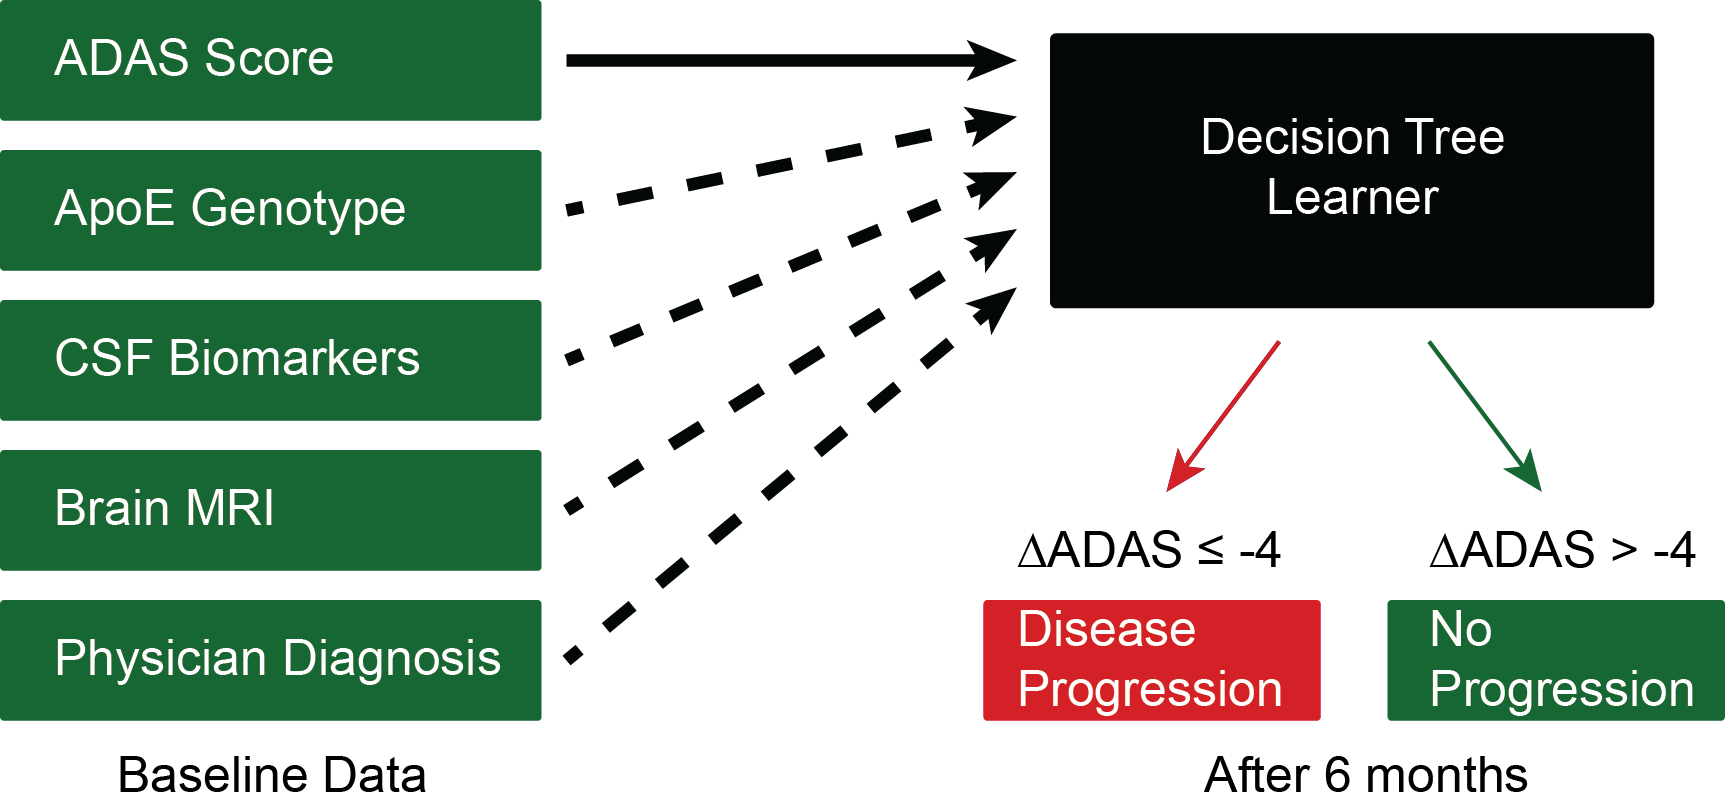
\includegraphics[width=.5\textwidth]{ADNIFlowchart.png}
    \caption{An illustration of the classification approach using ADAS-cog to quantify disease progression. For any given patient, data may be available for their ApoE Genotype, CSF Biomarkers, Brain MRI, and Physician Diagnosis, but the ADAS score at baseline is always included.}
\end{figure}


\section{Results}
% this is what we learned about the data


% this is our result from trying a Regression algorithm
\subsection{Linear Regression with MMSE as output}
With an 80:20 training/testing split, the linear regression predictor explained 60\% of the variance in our $(\Delta$MMSE$)$. The residual sum of squares was 10.42.

\subsection{Classification Algorithms with MMSE as output}
After switching to a classification problem, we were able to obtain somewhat better results, while still using MMSE to quantify disease progression (Table 3). We tried five different classification algorithms, SVM, K-Nearest Neighbors, Naive Bayes, Decision Trees and ADABoost, on different parameters. The SVM  model with a penalty of 0.1 and a linear kernel gave us the best results, with a training accuracy of $64.4\%$ and testing accuracy of $67.5\%$. 
%SVM results
%Decision Tree Results
%Naive Bayes
\begin{table}[h]
\caption{Classification accuracies for different variations the machine learning models SVM, Decision Trees, and Naive Bayes on dataset categorized by MMSE labels from Table 1.}
\label{sample-table}
\vskip 0.15in
\begin{center}
\begin{small}
\begin{sc}
\begin{tabular}{lcccr}
\hline
\abovespace\belowspace
Model & & Params & Train & Test Acc. \\
\hline
\abovespace
SVM    & C = 0.1 & Linear & 64.4\% & 67.5\% \\
SVM    & C = 3 & Linear & 62.8\% & 66.2\% \\
SVM    & C = 0.5 & Gauss & 70.0\% & 65.6\% \\
SVM    & C = 1 & Poly & 70.0\% & 61.0\% \\
K-NN    & K = 5 && 65.9\% & 65.6\% \\
N. Bayes    &Multi& & 62.5\% & 65.6\% \\
D. Trees    &Depth & 2 & 61.5\% & 65.6\% \\
\belowspace
Adaboost    & D.Tree  &  & 57.1\% & 59.7\% \\
\hline
\end{tabular}
\end{sc}
\end{small}
\end{center}
\vskip -0.1in
\end{table}
%include enough detail that someone could re-produce the result
%create one key figure
%List metrics of the various algorithms in a table format

\subsection{Decision tree classification with ADAS-cog as output}
%INCLUDE RESULTS ABOUT OUR DT WORK FROM TODAYYYYYYY!Y!Y!Y!


\section{Next Steps}
\subsection*{Enlarging the dataset}
This approach could be applied to the ADNI GO and ADNI 2 datasets, which are extensions of the data investigated here in some ways. They have many features in common, but also include additional features which may also be informative. In the future, we could include data from a study done in 2012, the AddNeuron trial. This includes additional clinical evidence and better genomic features. Furthermore, we are also considering complementing our database with the Penn AD Core Center database. Namely, we want to look specifically at some of the genome sequencing data to attempt to derive meaning from imputed genomes, and determine if genes besides ApoE would inform our predictions.

\section{Discussion}
Our first few attempts to create a useful algorithm resulted in little success but much insight into the importance of domain specific knowledge in machine learning. Initially, we quantified progression using a regressor to predict an MMSE numerical value after 24 months. This was misguided because clinicians are more interested in using MMSE to categorize patients by the severity of their dementia, as opposed to pinning down an exact MMSE number. So, we classified patients into four cognitive state classes by MMSE and achieved test accuracies $>$ 65\%. Upon discussing this work with specialist physician-scientists, we determined that AD drug developers and doctors would be more interested in a classifier that quantified AD progression with the ADAS-cog test. We also included new features that are thought to be informative, including CSF biomarkers and MRI quantification of brain morphology, as well as physician's holistic diagnoses. After pre-screening this new dataset for the highest standard of QC, we determined to use a decision tree to classify patients disease progression, using their baseline data.

The decision tree was an appropriate learning algorithm for several reasons. They are strong performers for mixed data types, handle missing values well, are robust to outliers, scale easily, handle irrelevant inputs, and are mostly interpretable.  It was crucial that our system have a high degree of interpretability, given that we aspire to apply it in a clinical setting to aid physicians in their decision-making. They would not be likely to accept a "black box" algorithm. Also, ADNI data and other AD patient databases often include irrelevant features. Here, we pre-screened the data to ensure all features' relevance, but others may not follow the same procedures, so it is useful to use an algorithm that can appropriately ignore such features. Since the data comes from several institutions there are sometimes discrepancies in which features are reported for a given patient. Decision trees can handle such missing values at a node by assigning the most common value of all examples sorted to that node, for example. Other methods can also handle this issue effectively.

%%%NEED TO TALK MORE HERE ABOUT THE DECISION TREE"S ACTUAL RESULTS. COMPARE THE DIFFERENT COMBINATIONS OF DATA GROUPS AND DISCUSS WHICH ONES ARE MOST IMPORTANT AND WHICH HAVE LITTLE BENEFIT.





%\subsection{Citations and References} 
%
%Please use APA reference format regardless of your formatter
%or word processor. If you rely on the \LaTeX\/ bibliographic 
%facility, use {\tt natbib.sty} and {\tt icml2014.bst} 
%included in the style-file package to obtain this format.
%
%Citations within the text should include the authors' last names and
%year. If the authors' names are included in the sentence, place only
%the year in parentheses, for example when referencing Arthur 
%'s
%pioneering work %\yrcite{Samuel59}. Otherwise place the entire
%reference in parentheses with the authors and year separated by a
%comma %\cite{Samuel59}. List multiple references separated by
%semicolons \cite{kearns89,Samuel59,mitchell80}. Use the `et~al.'
%construct only for citations with three or more authors or after
%listing all authors to a publication in an earlier reference \cite{MachineLearningI}.
%
%The references at the end of this document give examples for journal
%articles \cite{Samuel59}, conference publications \cite{langley00}, book chapters \cite{Newell81}, books \cite{DudaHart2nd}, edited volumes \cite{MachineLearningI}, 
%technical reports \cite{mitchell80}, and dissertations \cite{kearns89}. 
%
%Alphabetize references by the surnames of the first authors, with
%single author entries preceding multiple author entries. Order
%references for the same authors by year of publication, with the
%earliest first. Make sure that each reference includes all relevant
%information (e.g., page numbers).

 
\section*{Acknowledgments} 
 
We would like to thank Dr. Leslie Shaw and Dr. John Trojanowski for their advice on the best usage of the database and the relationship between the data features and the disease, especially with regards to CSF biomarkers and MRI data. Dr. Jon Toledo's help in selecting critical datasets of high quality from the large ADNI database was invaluable. 

Data collection and sharing for this project was funded by the Alzheimer's Disease Neuroimaging Initiative (ADNI) (National Institutes of Health Grant U01 AG024904) and DOD ADNI (Department of Defense award number W81XWH-12-2-0012). ADNI data are disseminated by the Laboratory for Neuro Imaging at the University of Southern California.

\bibliography{status}
\bibliographystyle{icml2014}

\end{document} 

%Have to Compile in BibTeX THEN LaTeX to get the references to show up for some reason (at least for Josh)


% This document was modified from the file originally made available by
% Pat Langley and Andrea Danyluk for ICML-2K. This version was
% created by Lise Getoor and Tobias Scheffer, it was slightly modified  
% from the 2010 version by Thorsten Joachims & Johannes Fuernkranz, 
% slightly modified from the 2009 version by Kiri Wagstaff and 
% Sam Roweis's 2008 version, which is slightly modified from 
% Prasad Tadepalli's 2007 version which is a lightly 
% changed version of the previous year's version by Andrew Moore, 
% which was in turn edited from those of Kristian Kersting and 
% Codrina Lauth. Alex Smola contributed to the algorithmic style files.  
